\documentclass[a4paper,11pt]{scrartcl}

\usepackage[english]{babel}

\usepackage[utf8]{inputenc} 
\usepackage[T1]{fontenc}
\usepackage{lmodern, mathpazo}
%\usepackage{helvet}
\usepackage{csquotes}
%\usepackage{musixtex}

\usepackage{amsmath, amsfonts, mathtools, amssymb}

\usepackage{etex}

\usepackage{tikz}
\usepackage{tikz-network}
\usepackage{hyperref}
\usepackage[english, nameinlink, noabbrev]{cleveref}
\usepackage[
    backend=biber,
    bibencoding=utf8,
    sorting=none,
    url=false,
    doi=false
]{biblatex}
\addbibresource{uni23.bib}

\usepackage{listings}

\usepackage{siunitx}
%\usepackage[onehalfspacing]{setspace}
\usepackage{graphicx}                   % Bilder
%\usepackage{floatflt}               % flt 
\usepackage{float}
\usepackage{physics}

\usepackage{caption}

\usepackage{amssymb}
\usepackage{amsmath}
%\usepackage{pgfplots}

\author{f}
\RequirePackage{etex}
\title{Review of results}
%\date{\today}

\begin{document}
\maketitle
\section{Introduction}
In \citeyear{BA_Pendry_1983}, \citeauthor{BA_Pendry_1983} derived a bound on the flow of information, which reads
\begin{align}\label{eq:pendry}
    \dot{I}^2 \leq \frac{\pi}{3\hbar\ln^22}\dot{E}.
\end{align}
This result is derived using classical statistical mechanics \cite{BA_Pendry_1983}. This classical framework, however,
neglects the effects of genuine quantum mechanical phenomena, such as quantum correlations. We show that this
classical inequality is violated when in a system with quantum correlations.
\section{The model}
Consider a chain of qubits in the Heisenberg-$XY$ model. Restricting their interaction to their nearest neighbors allows
us to draw a comparison to Pendry's original derivation with fermions using Jordan-Wigner transform, mapping a chain of
spin-$1/2$ qubits to a chain of spinless fermions. The information flow is then the time derivative of 

In particular, we have the Hamiltonian of this system as
\begin{align}\label{eq:hamiltonian-perfect-transfer}
    H &= \sum\limits_i \sigma^z_i + \sum\limits_k \frac{J_k}{2} (\sigma^x_k\sigma^x_{k+1}+\sigma^y_k\sigma^y_{k+1})\\
    \shortintertext{with}\\
    J_k &= \frac{\lambda}{2}\sqrt{k\cdot(N-k)}.\nonumber
\end{align}
This ensures a predictable periodic behaviour of the chain. This can be made apparent by considering the local
magnetization $\expval{\sigma^z_k}$ of the qubits. \Cref{fig:no-corr} shows the time evolution of the quibts'
magnetization.\footnote{We choose $\lambda$ to be $1$. It was shown in \cite{BA_Christandl_2004} that at
time $t=\pi/\lambda$, perfect state transfer is achieved}

\begin{figure}[H]
    \centering
    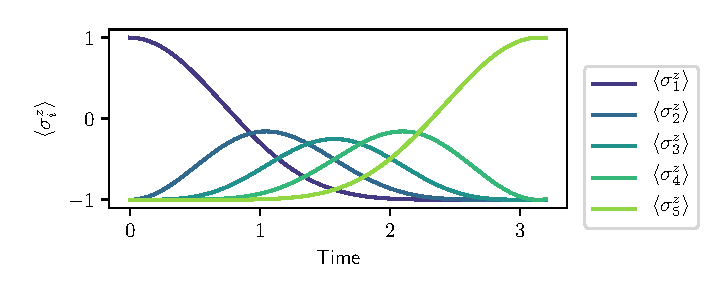
\includegraphics{expval_z.pdf}
    \caption{Time evolution of the individual magnetizations $\expval{\sigma^z_i}$ for the system with
    Hamiltonian defined as in \cref{eq:hamiltonian-perfect-transfer}.
    Qubit $i=1$ is prepared in the excited state at time $t=0$.
    Qubits $i>1$ are prepared in the ground state at time $t=0$.}
    \label{fig:no-corr}
\end{figure}
\section{Quantum correlations}
In a work by \citeauthor{BA_kaonan_correlations}, it was shown that certain quantum correlations
\emph{invert} the flow of energy \cite{BA_kaonan_correlations}. Heat flows not from hot to cold, but
from cold to hot. \Cref{fig:corr} shows the chain with inital correlations at positions 1 and 2 of the chain.
%\begin{figure}
%    \centering
%\end{figure}


%\begin{displayquote}
%Since energy is conserved the flow into this segment equals the
%flow out and therefore energy flow is conserved as is the particle flow. However,
%the entropy flow is not conserved but can only increase monotonically until thermal
%equilibrium is established.
%\end{displayquote}


\printbibliography
\end{document}
